\section{Build Jobs}

''Build jobs'' predstavlja skup poslova u koji spadaju kompajliranje, testiranje, pakovanje, razvijanje projekta ili bilo koji drugi posao koji manevriše sa vašim projektom. ''Build job'' je osnovni pojam kad se govori o principu kontinualne integracije.

\subsection{Kreiranje Build Job-a}

Pravljenje ''build job-a'' je veoma jednostavno i ono podrazumeva razna podešavanja. Prvo treba odrediti kakvog će tipa biti projekat. Postoji pet osnovnih i to su:
\begin{itemize}  
\item Slobodan projekat(Freestyle software project) - Vrsta projekta koji pružaju maksimalnu fleksibilnost i koji služe za osnovnu upotrebu
\item Maven project - ''build job'' koji je specijalno namenjen Maven projektima
\item External job - ova opcija služi da se prate izvršavanja nekog drugog procesa koji se ne nalazi na Jenkins-u
\item Multi-configuration project - ova opcija je pogodna za projekte koji zahtevaju više različitih konfigurisanja
\item Copy existing job - projekat može da bude i kopija već postojećeg projekta koji zahteva neke promene u konfigurisanju
\end{itemize}  

\subsubsection{Kreiranje slobodnog projekta}

Slobodan projekat je najfleksibilnija vrsta i može se koristiti za bilo koju vrstu projekta. Puno opcija koje se nameštaju u okviru slobodnog projekta se javljaju i u ostalim vrstama projekta. Pri kreiranju projekta prvo se unose osnovni podaci kao što su ime projekta i opis projekta. Zatim slede opcije:

\begin{itemize}  
\item Discard Old Builds - čekiranjem ove opcije limitirate broj bildova koji će se čuvati, postoje dva kriterijuma:
\begin{itemize}
\item Po starosti - bild se briše posle određenog vremena
\item Po broju - čuva se N bildova
\end{itemize}
\item This build is parameterized - korisnik dodeljuje parametre koje će bild koristiti. Neki od parametara su:
\begin{itemize}
\item Boolean Parameter - definiše se string ''true'' ili ''false'' koji se može koristiti u procesu bildovanja
\item Choice Parameter - definiše se string koji može imati bilo koju vrednost iz liste izbora i koji se može koristiti u procesu bildovanja
\item Password Parameter - definiše se tekst gde korisnici mogu da unesu string vrednost koji se može koristiti tokom proces bildovanja
\end{itemize}
\item Disable Build - kad je čekirano privremeno se obustavlja bildovanje
\item Execute concurrent builds if necessary - čekiranjem ove opcije, omogućava se paralelno izvršavanje bildovanja. Veoma kosrisno kod parametrizovanih bildova gde su izvršavanja nezavisna jedna od drugih
\end{itemize}

''Napredne'' opcije:
\begin{itemize}  
\item Quiet period - čekiranjem ove opcije, zadaje se broj sekundi nakon koliko će se pokrenuti sledeći bild
\item Retry Count - u slučaju da bild ne uspe, zadaje se broj ponovnih pokušaja
\item Block build when upstream project is building - sprečava se bildovanje ako je neki projekat od koga je zavistan trenutni projekat isto u procesu bildovanja
\item Block build when downstream project is building - sprečava se bildovanje ako je neki projekat koji je zavistan od trenutnog isto u procesu bildovanja
\item Use custom workspace - manualno zadavanje radnog prostora
\end{itemize}

\subsection{Integracija sa izvornim kodom}

Jedna od najbitnijih i najznačajnijih stvari je integracija sa sistemom za kontrolu verzija. Jenkins prati svaku promenu u vašem izvornom kodu posle kojih se pokreće kompajliranje i razni automatski testovi. Podržani su razni sistemi za kontrolu verzija, CVS i Subversion ''u startu'', dok za sisteme kao što su Git, Mercurial, Harvest, BitKeeper i ostale postoje plugin-ovi koji se lako instaliraju preko Jenkins plugin Manager-a. Pri pravljenju projekta i odabiru koji sistem za kontrolu verzija će se koristiti, unošenjem URL-a repozitorijuma se vrši integracija sa izvornim kodom.

\subsection{Git Setup}

Da bismo mogli da se povežemo sa Git-om prvo moramo instalirati Git. Za operativne sisteme Windows i Mac OS postoje instalacije, a na Linuxu se instalira putem jednostavne komande:

\begin{verbatim}
 sudo apt-get install git-all
\end{verbatim}

Za razliku od sistema za kontrolu verzija kao što su CVS i Subversion čiji su plugin-ovi već instalirani, plugin za Git, koji se nalazi u Jenkins-ovom plugin Manager-u, morate sami instalirati. Nakon instalacije pri pravljenju novog projekta, u opcijama za biranje sistema za kontrolu verzija otvoriće se opcija i za Git što je prikazano na slici \ref{fig:git}

\begin{figure}[h!]
\begin{center}
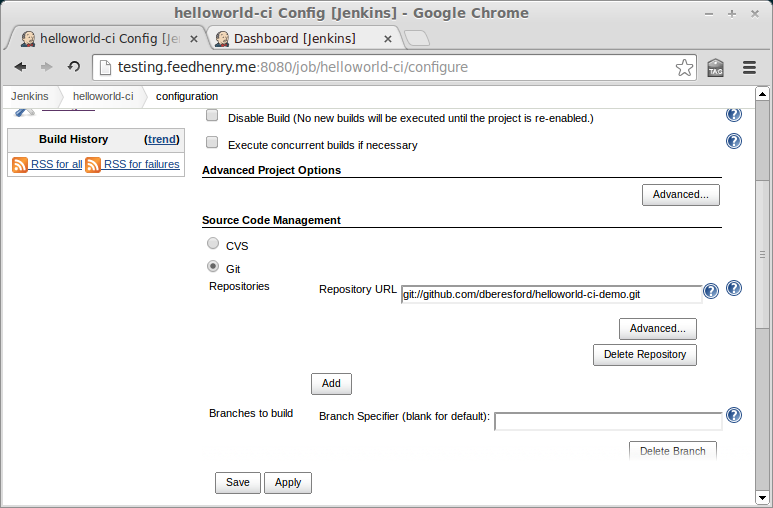
\includegraphics[scale=0.75, totalheight=0.4\textheight]{slike/git_jenkins.png}
\end{center}
\caption{Git}
\label{fig:git}
\end{figure}

Uz opcije ''Repository'' gde se navodi URL repozitorijuma i ''Branches to build'' gde se navodi ime branch-a(grane) koje se bilduje postoje i tzv. ''Dodatna ponašanja''(Additional Behaviours). Neka od njih su:
 
\begin{itemize}  
\item Polling ignores commits from certain paths
\begin{itemize}
\item Included regions - unose se putanje fajlova koje se bilduju
\item Excluded regions - unose se putanje fajlova čije testiranje nema efekta npr. slike
\end{itemize}
\item Polling ignores commits in certain users 
\begin{itemize}
\item Excluded users - imena user-a od čije strane ne može da se pokrene bildovanje
\end{itemize}
\end{itemize}

\subsection{Pokretanje bildova}

Nakon nameštanja koji ćete sistem za kontrolu verzija koristiti, vreme je da se konfiguriše kada će se bildovi pokretati. Postoje osnovne tri vrste pokretanja bildova, a to su:

\begin{itemize}
  
\item Build after other projects are built - ova opcija pruža pokretanje bilda kad god se neki drugi bild izvrši. Postoje i 3 dodatne opcije:
\begin{itemize}  
\item Trigger only if build is stable - pokreni bild samo ako je bild stabilan
\item Trigger even if the build is unstable - pokreni bild iako je bild nestabilan
\item Trigger even if the build fails - pokreni bild iako bild ne uspe
\end{itemize}

\item Build periodically

Odlika kontinualne integracije jeste kontinualno izvršavanje bildovanja nakon svake promene što nije stvar kod periodičnog bildovanja. U nekim slučajevima je i pogodno koristiti ovu vrstu pokretanja npr. kod projekata gde iscrpna testiranja traju i po nekoliko sati i gde je pogodnije pokretati bildove u određenim vremenskim intervalima.
Sintaksa za zadavanje vremenskog intervala: \\
MINUTE HOUR DOM MONTH DOW
\begin{itemize}
\item MINUTE - minut u satu (0-59)
\item HOUR - sat u danu (0-23)
\item DOM - dan u mesecu (1-31)
\item MONTH - mesec(1-12)
\item DOW - dan u nedelji(0-7) gde su 0 i 7 nedelje
\end{itemize}

\item Poll SCM

Bolja strategija od periodičnog bildovanja jeste Polling the SCM tzv. ''ispitivanje'' sistema za kontrolu verzija. Ideja je da se sistem za kontrolu verzija ''ispituje'' da li je napravljena izmena u izvornom kodu. U slučaju da jeste Jenkins će pokrenuti bild.
\end{itemize}

\subsection{Koraci bildovanja}

Definisanjem bild koraka govorite Jenkins-u šta da radi sa vašim izvornim kodom. Jedan bild može da ima više koraka u koje spadaju izvršavanje shell skripte, izvršavanje Windows batch komande ili povezivanje sa Maven-om ili Ant-om.

\subsection{Akcije posle bildovanja}

Nakon samog procesa bildovanja potrebno je preduzeti neke akcije. Neke od mogućih akcija su:
\begin{itemize}
\item Archive the artifacts - ova opcija omogućava da se rezultati bildovanja čuvaju u određenom formatu i da se zatim downloaduju
\item E-mail Notifications - Jenkins obaveštava mejlom svaki put kada bild ne uspe, kada uspe bild nakon neuspelog pokušaja, kada je build nestabilan nakon uspešnog bildovanja.
\end{itemize}
